\documentclass{beamer}
\usetheme{Boadilla}
\usepackage{graphicx}
\graphicspath{{./images/}}
\usepackage{latexsym,amsmath,amssymb,amsthm,enumerate,mathrsfs,hyperref}
\newcommand{\Z}{\mathbb{Z}} % use \Z for the set of integers
\newcommand{\Q}{\mathbb{Q}} % use \Q for the set of rational numbers
\newcommand{\R}{\mathbb{R}} % use \R for the set of real numbers
\newcommand{\C}{\mathbb{C}} % use \C for the set of complex numbers
\newcommand{\N}{\mathbb N} % use \N for the set of natural numbers
\newcommand{\ps}{\mathcal P} % use \ps for the power set
\newcommand{\twomat}[4]{\displaystyle{\left[\begin{array}{cc}#1&#2\\#3&#4\end{array}\right]}}% for 2 by 2 matrices


%%%%%%%%%%%%%%%%%%%%%%%%%%%%%%%%%%%%%%%%%%%%%%%%%%%%%%%%%%%%%%%%%%%%%%%%%%%%%%%%%%%%

\title{Math351 Project: Algebraic Coding Theory}
\author{John Chu, Hieu Nguyen}
\institute{Dickinson College}
\date{\today}

\begin{document}

\begin{frame}
\titlepage
\end{frame}

\begin{frame}
\frametitle{Outline}
\tableofcontents
\end{frame}

%%%%%%%%%%%%%%%% Introduction %%%%%%%%%%%%%%%%%%%%%%%%

\section{Introduction}
\subsection{What is Algebraic Coding Theory?}
\subsection{Examples} %Barcode, John's examples%


\begin{frame}
\frametitle{What is Algebraic Coding Theory?}
\begin{Definition}
{Algebraic coding theory is a branch of mathematics concerned with the development of error-control codes and encoding/decoding techniques.}
\end{Definition}
\end{frame}

\begin{frame}
\frametitle{Real-Life Example}
\centering
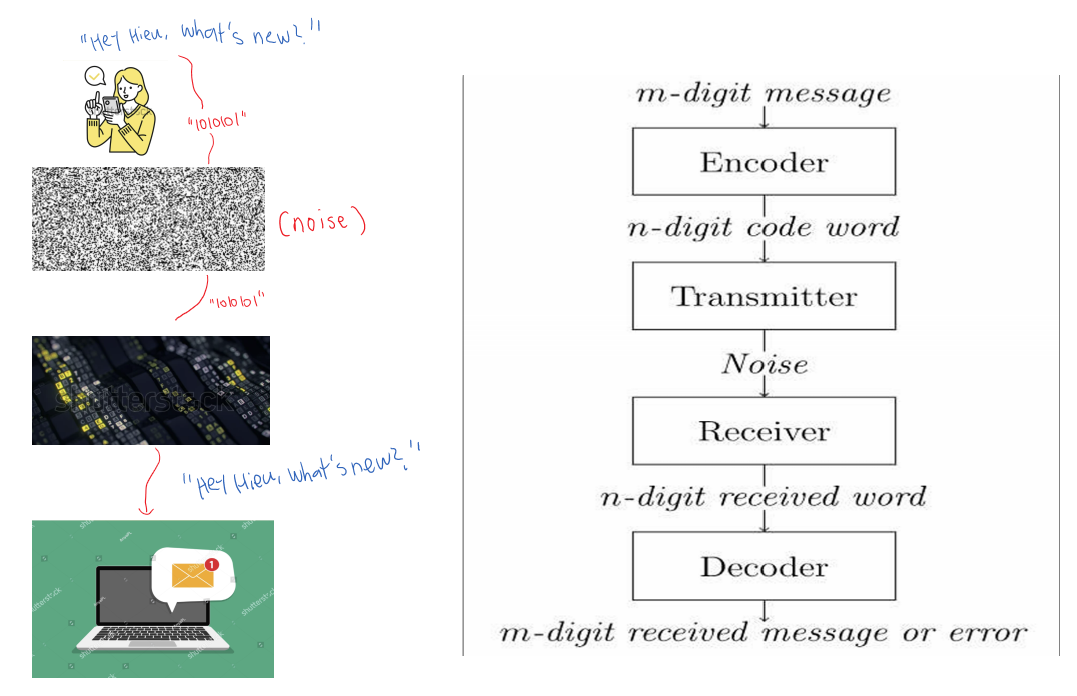
\includegraphics[scale=0.55]{images/hi1.png}
\end{frame}


%%%%%%%%%%%% Structure of codes, Error-detecting %%%%%%%%%%%%%%

\section{Basic mechanism: Code structure}
\subsection{Block code: encoding/decoding functions, codeword}
\subsection{Group codes, linear codes}

\begin{frame}{Basic Mechanism: Block Codes, Encoding/Decoding function}
\begin{Definition}
{A code is an $(n,m)$-block code if the information that is to be coded can be divided into blocks of $m$ binary digits, each of which can be encoded into $n$ binary digits}
\end{Definition}

\begin{exampleblock}{Encoding function}
    {
    E: Z_2^m \xrightarrow[]{} Z_2^n
    }
\end{exampleblock}

\begin{exampleblock}{Decoding function}
  {
  D: Z_2^n \xrightarrow[]{} $Z_2^m$
  }
\end{exampleblock}
\end{frame}

\begin{frame}
\frametitle{Code structure: Group codes}
\begin{Definition}
{Group code is a code that is also a subgroup of \Z_2^n.}
\end{Definition}

\begin{itemize}
    \item{
    To verify the group code,  add every codeword to its own inverse and produces 0.
    }
    \item{11000101 + 11000101 = 0000000 (group code)}
\end{itemize}

\begin{exampleblock}{Example}
Suppose that we have a code that consists of the following 7-digits \\
\centering
    \begin{matrix}
    (0000000) & (0001111) & (0010101)  & (0011010) \\
    (0100110) & (0101001) & (0110011)  & (0111100) \\
    (1000011) & (1001100) & (1010110)  & (1011001) \\
    (1100101) & (1101010) & (1110000)  & (1111111) \\
    \end{matrix}
\end{exampleblock} 
\end{frame}

\begin{frame}
\frametitle{Recall}
\begin{itemize}
    \begin{exampleblock}
        {Null Space}
        {A matrix $H \in M_{m \times n}(Z_2)$ such that $Hx = 0$}
    \end{exampleblock}
    
    \begin{exampleblock}
        {Inner Product}
        {Inner product is a dot product of each binary digit such that $x \cdot y = x_1y_1 + \cdots + x_ny_n$ for binary $x,y \in M_{m \times n}$}
    \end{exampleblock}
\end{itemize}

\end{frame}

\begin{frame}
\frametitle{Code structure: Linear codes}
\begin{Definition}
{Linear Code is a code that is determined by the null space.}
\end{Definition}
    
\begin{exampleblock}
    {Application Example}
    Suppose x = (010011)^t. 
    \centering
    {H = \begin{bmatrix}
    0 & 0 & 0 & 1 & 1 & 1 \\
    0 & 1 & 1 & 0 & 1 & 1 \\
    1 & 0 & 1 & 0 & 1 & 1 \\
    \end{bmatrix}} \\
    Then, notice that $Hx = \begin{bmatrix}
    0 \\
    1 \\
    1 \\
    \end{bmatrix} \neq 0$. \\
    Thus, received text is not a codeword
\end{exampleblock}


\end{frame}


%%%%%%%%%% Parity-check and generator matrices %%%%%%%%

\section{Check linear code and encoding}
\subsection{Error coding schemes: repetition, even parity}
\subsection{Abstract algebra behind the parity-check}

\begin{frame}{A crude error coding scheme}
    \begin{exampleblock}{Repetition: Comparison of multiple copies of encoded messages}
        Suppose that the message to be encoded is a binary $n$-row. The message is encoded into a binary $n$-tuple by simply repeating the message three times\\
        $(x_1,x_2,..., x_n)\rightarrow (x_1, x_2,..., x_n, x_1, x_2, ... x_n, x_1, x_2, ..., x_n)$\\
        Original message: $(0110)$ \\
        Repeated codeword: $(0110\text{ }1110\text{ } 0110)$\\
        The transmission error in the 5th digit, so the correctly decoded message can be assumed to be $(0110)$
    \end{exampleblock}  
    In reality, this method is slow! 
\end{frame}

\begin{frame}{More efficient error coding scheme: Even parity}
    \begin{exampleblock}{Even parity: Checking the number of 1s in a codeword}
        There are $2^7=128$ ASCII characters, but the whole coding system has $2^8=256$ possible characters with $0$ always on the far left. For example, 
        \begin{align*}
        A=65_{10}=01000001_2, C=01000011_2    
        \end{align*}
        Even parity first forces each character to have an even number of 1s. That is, 
        \begin{align*}
            A=01000001_2, C=11000011_2
        \end{align*} where $C$ has to replace the far left $0$ with $1$ to have an even number of $1s$. Suppose an A is sent and a transmission error in the sixth bit is caused by noise over the communication channel so that $(0100\text{ }0101)$ is received. There is an error because there are an odd number of 1s. 
    \end{exampleblock}
    More efficient and commonly used.
\end{frame}

\begin{frame}{Understanding the abstract algebra of the parity check}
\begin{itemize}
  \item \textbf{Canonical parity-check matrices}\\
  $H=(A|I_m)$ where $A$ is the $m\times(n-m)$ matrix
  \begin{align*}
    \begin{pmatrix}
        a_{11} & a_{12} & \dots & a_{1,n-m} \\
        a_{21} & a_{22} & \dots & a_{2,n-m} \\
        \vdots & \vdots & \ddots & \vdots \\
        a_{m1} & a_{m2} & \dots & a_{m,n-m}
    \end{pmatrix}
      \end{align*}
     and $I_m$ is the $m\times m$ identity matrix
  \item For each canonical parity-check matrix we can associate an $n\times (n-m)$ \textbf{standard generator matrix}:
  \[
      G=\left( \displaystyle{\frac{I_{n-m}}{A}} \right)
    \]
\end{itemize}
\end{frame}

\begin{frame}{Theorem basis and meaning}
\begin{theorem}
If $H\in M_{m\times m}(\Z_2)$ is a canonical parity-check matrix, then Null($H$) consists of all $x\in \Z_2^n$ whose first $n-m$ bits are arbitrary but whose last $m$ bits are determined by $Hx=0$. Each of the last $m$ bits serves as an even parity check bit for some of the first $n-m$ bits. Hence, $H$ gives rise to an $(n, n-m)$-block code. 
\end{theorem}
\begin{theorem}
Let $H=(A|I_m)$ be an $m\times n$ canonical parity-check matrix and $G=\left( \displaystyle{\frac{I_{n-m}}{A}} \right)$ be the $n\times (n-m)$ standard generator matrix associated with $H$. Let $C$ be the code generated by $G$. Then $y$ is in $C$ iff $Hy=0$. So, $C$ is a linear code with canonical parity-check matrix $H$.
\end{theorem}
Check the linear code!
\end{frame}

\begin{frame}{Criteria for a single error-correcting code}
\begin{theorem}
The null space of $H$ is a single error-correcting code iff $H$ does not contain any zero columns and no two columns of $H$ are identical. 
\end{theorem}
\begin{exampleblock}{Example}
        Consider $H_1$=\begin{pmatrix}
                1 & 1 & 1 & 0 & 0 \\
                1 & 0 & 0 & 1 & 0 \\
                1 & 1 & 0 & 0 & 1 \\
        \end{pmatrix},
        $H_2$=\begin{pmatrix}
                1 & 1 & 1 & 0 & 0 \\
                1 & 0 & 0 & 0 & 0 \\
                1 & 1 & 0 & 0 & 1 \\
        \end{pmatrix}. \\
Note that the null space of $H_1$ is a single error-detecting code while $H_2$ is not. 
\end{exampleblock}
\end{frame}

%%%%%%%%%%%%%%%%%% Efficient decoding %%%%%%%%%%%%%%%%%

\section{Efficient decoding scheme}
\subsection{Determine codeword, coset decoding, syndrome, decoding table}

\begin{frame}{Coset decoding}
\begin{Definition}
Suppose that C is an $(n,m)$ linear code. A coset of $C \in Z_2^n$ is written as x + C and we have $2^{n-m}$ distinct cosets by Lagrange's Theroem. 
\end{Definition}

\begin{itemize}
    \item {
        Coset can be usefully applied for coset decoding. 
    }
    
    \item{
        Given receiver code r, we can compute what sender code s is.
    } 
    
    \item{
        To decode r, find in which coset element that r \in x + C
    }\\
    
\end{itemize}
\end{frame}

%%%%%%%%%%%%%%%%%%%%%%%Decoding Example %%%%%%%%%%%%%%%%%%%%%
\begin{frame}
\frametitle{Decoding Example}
\begin{exampleblock}
{Example}
{Let H be a (5,3) matrix such that H = 
\begin{bmatrix}
0 & 1 & 1 & 0 & 0 \\
1 & 0 & 0 & 1 & 0 \\
1 & 1 & 0 & 0 & 1 \\
\end{bmatrix} \\
Then, code consist of codewords (00000), (01101), (10011), (11110). \\
Then, the coset is as follows: \\
\centring
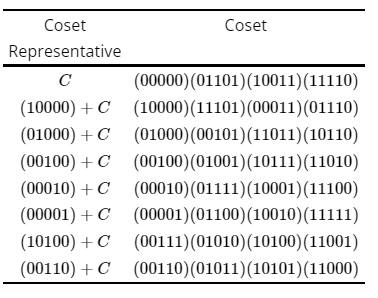
\includegraphics[scale=0.55]{images/Question3.png}
 }
\end{exampleblock}
\end{frame}

\begin{frame}
    \frametitle{Decoding Example}
    \begin{exampleblock}
    {Example}
    {Let the receiver code r = (01111). Note that $r \in (00010) + C$. 
    Therefore, (01111) + (00010) = (01101) = s
    }
    \end{exampleblock}
\end{frame}


%%%%%%%%%%%%%%%%%% Bibliography %%%%%%%%%%%%%%%%%%%%%%%%%%%%%%%%%%%

\begin{frame}
\frametitle{Bibliography}
\centering
https://www.shutterstock.com \\
Algebraic Coding Theory | Judson Chapter 8
    
\end{frame}

%%%%%%%%%%%%%%%%%% Thanks %%%%%%%%%%%%%%%%%%%%%%%%%%
\begin{frame}
    \begin{center}
        {\Huge Thank You}
    \end{center}
\end{frame}

\end{document}